\documentclass[tikz,border=6pt]{standalone}
% Shared visual language for the original benchmark atlas.
\usepackage[T1]{fontenc}
\usepackage{lmodern}
\usepackage{amsmath,amssymb}
\usetikzlibrary{arrows.meta,calc,positioning,shapes.geometric,patterns,decorations.pathmorphing,backgrounds,fit}
\definecolor{ink}{HTML}{173948}
\definecolor{flow}{HTML}{167D9A}
\definecolor{control}{HTML}{A65217}
\definecolor{measure}{HTML}{70518A}
\definecolor{pale}{HTML}{EAF2F5}
\definecolor{muted}{HTML}{526571}
\definecolor{utility}{HTML}{2E8665}
\tikzset{
  every node/.style={font=\sffamily\small,text=ink},
  equipment/.style={draw=ink,line width=1pt,fill=pale,rounded corners=2pt},
  process/.style={draw=flow,line width=1.2pt,-{Latex[length=2.5mm]}},
  signal/.style={draw=control,line width=.8pt,dashed,-{Latex[length=2mm]}},
  util/.style={draw=utility,line width=1pt,-{Latex[length=2.2mm]}},
  dimension/.style={draw=muted,line width=.6pt,{Latex[length=1.7mm]}-{Latex[length=1.7mm]}},
  labelbox/.style={fill=white,inner sep=2pt,font=\sffamily\footnotesize,align=center},
  annotation/.style={font=\sffamily\footnotesize,text=muted,align=left},
  panel/.style={draw=ink!20,fill=ink!2,rounded corners=3pt,inner sep=6pt},
  instrument/.style={circle,draw=measure,fill=white,line width=.8pt,minimum size=8mm,inner sep=1pt,font=\sffamily\scriptsize,align=center},
  port/.style={circle,fill=flow,inner sep=1.6pt},
  box/.style={equipment,minimum width=3cm,minimum height=1cm,align=center},
}
\newcommand{\atlasheader}[3]{%
  \node[anchor=north west,font=\sffamily\bfseries\LARGE] at (0,0) {#1};%
  \node[anchor=north west,font=\sffamily\small,text=muted] at (0,-.75) {Paper section #2: \textit{#3}};%
  \draw[ink!25,line width=.7pt] (0,-1.25)--(26,-1.25);%
}
\newcommand{\atlasfooter}[1]{%
  \draw[ink!25,line width=.5pt] (0,-15.8)--(26,-15.8);%
  \node[anchor=north west,annotation,text width=25.8cm] at (0,-16) {#1\\Original explanatory drawing. Source: Kroll \& Schulte (2014), DOI: 10.1016/j.asoc.2014.08.034. Model variants are identified in the accompanying case sheet.};%
}

\begin{document}
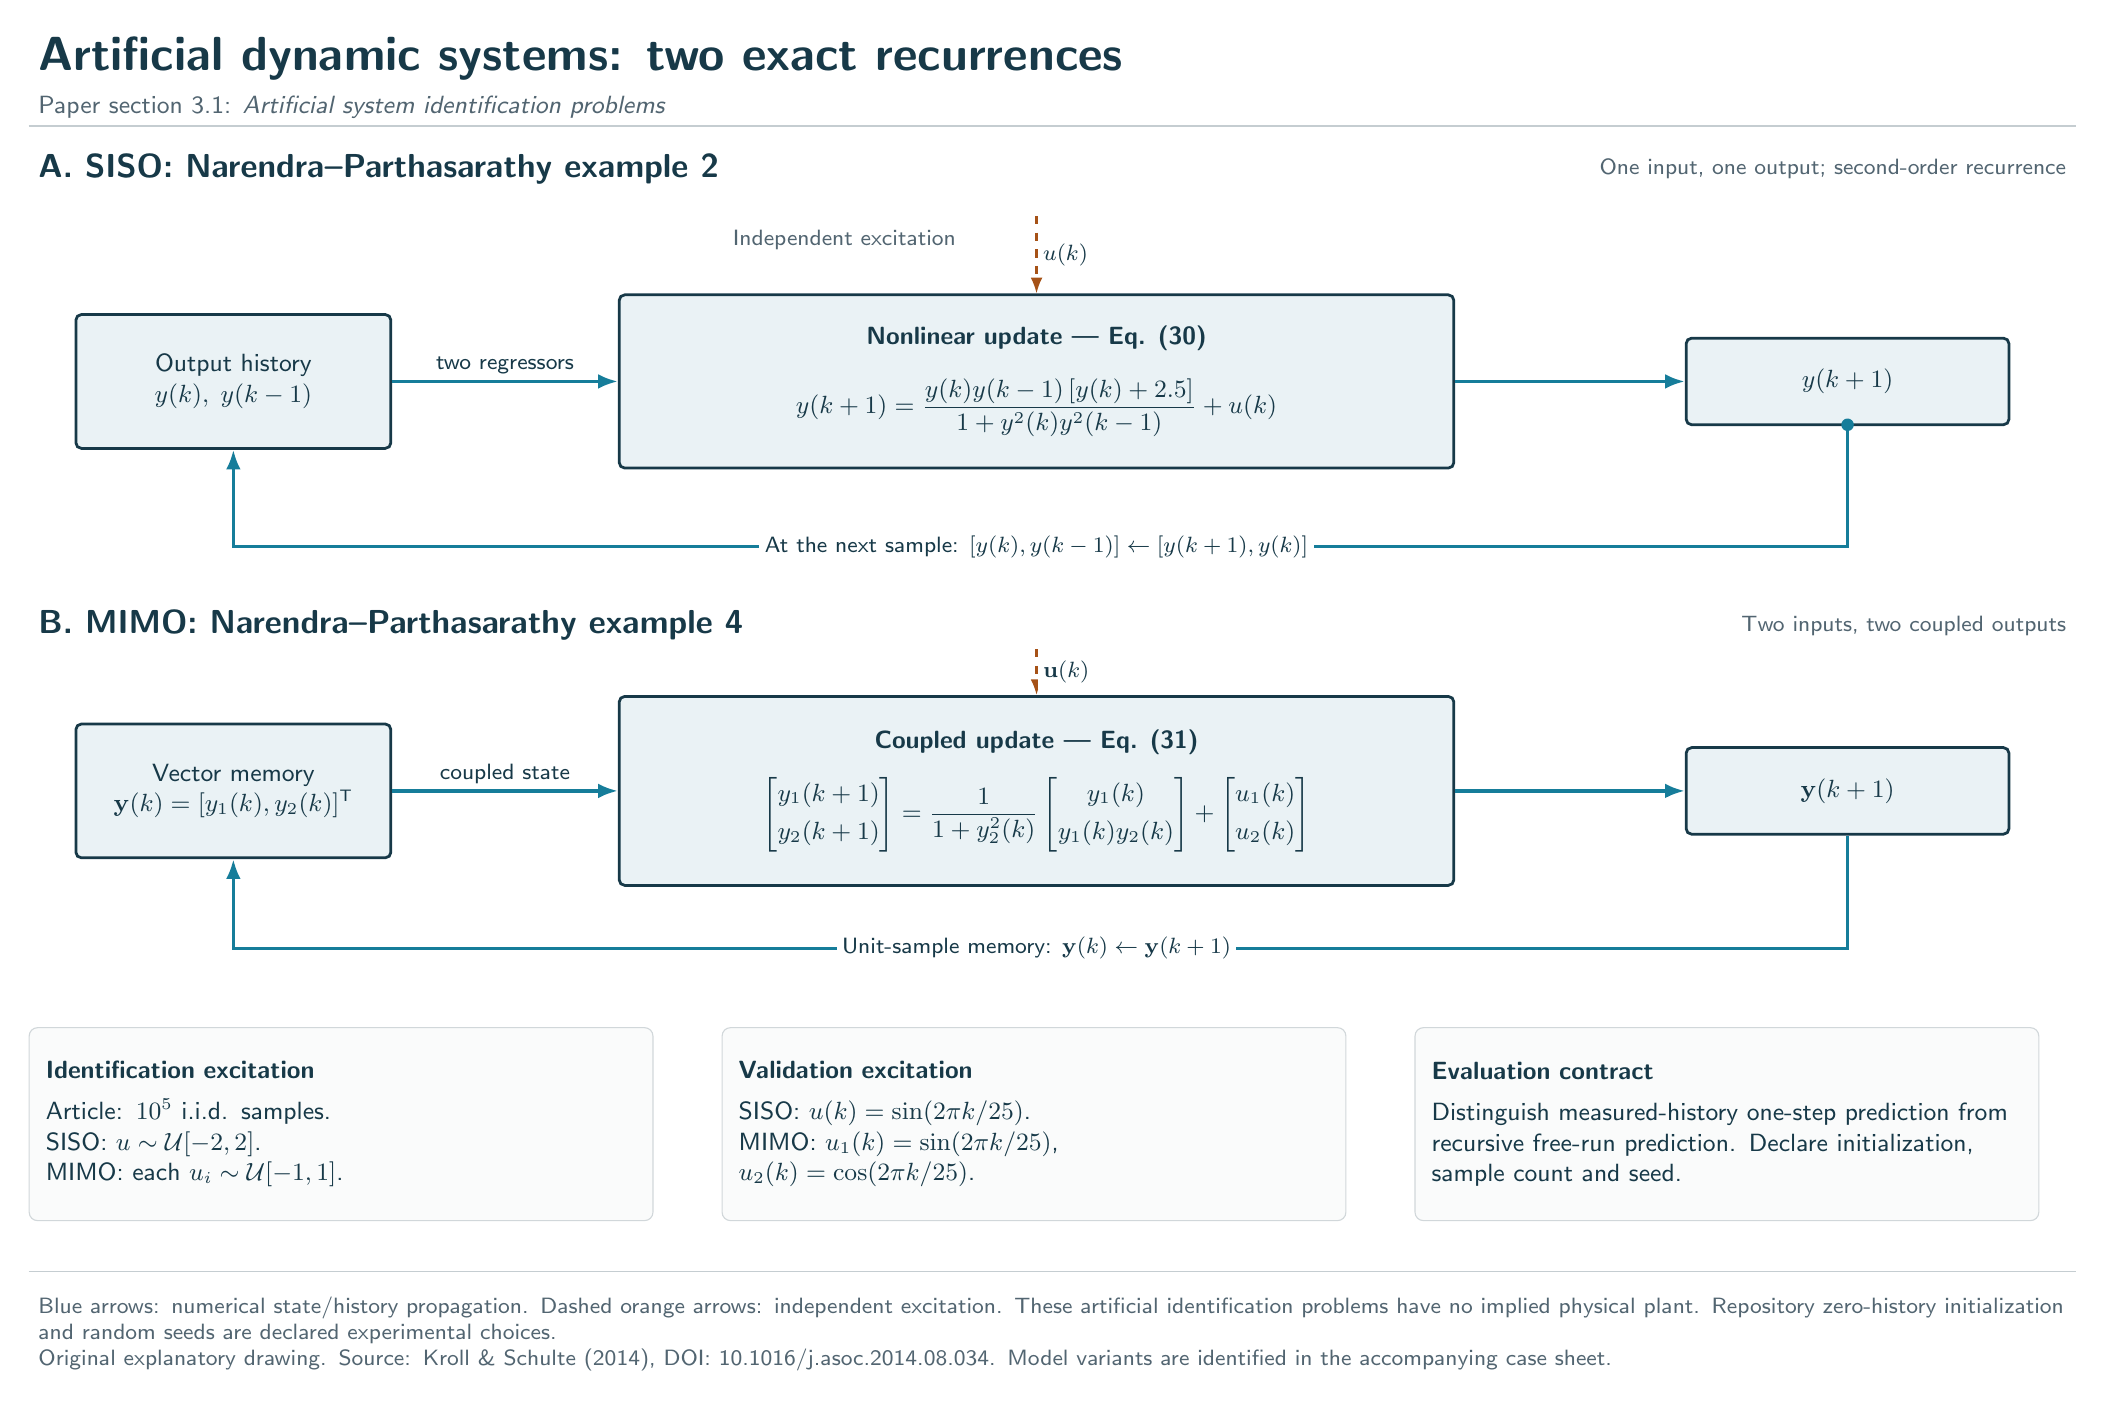
\begin{tikzpicture}[x=1cm,y=1cm]
\atlasheader{Artificial dynamic systems: two exact recurrences}{3.1}{Artificial system identification problems}
\node[anchor=west,font=\sffamily\bfseries\large] at (0,-1.8) {A. SISO: Narendra--Parthasarathy example 2};
\node[anchor=east,annotation] at (26,-1.8) {One input, one output; second-order recurrence};
\node[box,minimum width=4cm,minimum height=1.7cm] (sisoMemory) at (2.6,-4.5) {Output history\\$y(k),\;y(k-1)$};
\node[box,minimum width=10.6cm,minimum height=2.2cm] (siso) at (12.8,-4.5)
 {\textbf{Nonlinear update --- Eq. (30)}\\[9pt]
 $\displaystyle y(k+1)=\frac{y(k)y(k-1)\,[y(k)+2.5]}{1+y^2(k)y^2(k-1)}+u(k)$};
\node[box,minimum width=4.1cm,minimum height=1.1cm] (sisoOutput) at (23.1,-4.5) {$y(k+1)$};
\draw[process] (sisoMemory.east)--node[above,labelbox]{two regressors}(siso.west);
\draw[process] (siso.east)--(sisoOutput.west);
\draw[signal] (12.8,-2.4)--node[right,labelbox]{$u(k)$}(siso.north);
\node[anchor=east,annotation] at (11.9,-2.7) {Independent excitation};
\draw[process] (sisoOutput.south)--(23.1,-6.6)--(2.6,-6.6)--(sisoMemory.south);
\node[labelbox] at (12.8,-6.6) {At the next sample: $[y(k),y(k-1)]\gets[y(k+1),y(k)]$};
\node[port] at (23.1,-5.05) {};

\node[anchor=west,font=\sffamily\bfseries\large] at (0,-7.6) {B. MIMO: Narendra--Parthasarathy example 4};
\node[anchor=east,annotation] at (26,-7.6) {Two inputs, two coupled outputs};
\node[box,minimum width=4cm,minimum height=1.7cm] (mimoMemory) at (2.6,-9.7) {Vector memory\\$\mathbf y(k)=[y_1(k),y_2(k)]^\mathsf T$};
\node[box,minimum width=10.6cm,minimum height=2.4cm] (mimo) at (12.8,-9.7)
 {\textbf{Coupled update --- Eq. (31)}\\[7pt]
 $\displaystyle\begin{bmatrix}y_1(k+1)\\[3pt]y_2(k+1)\end{bmatrix}
 =\frac{1}{1+y_2^2(k)}\begin{bmatrix}y_1(k)\\[3pt]y_1(k)y_2(k)\end{bmatrix}
 +\begin{bmatrix}u_1(k)\\[3pt]u_2(k)\end{bmatrix}$};
\node[box,minimum width=4.1cm,minimum height=1.1cm] (mimoOutput) at (23.1,-9.7) {$\mathbf y(k+1)$};
\draw[process] (mimoMemory.east)--node[above,labelbox]{coupled state}(mimo.west);
\draw[process] (mimo.east)--(mimoOutput.west);
\draw[signal] (12.8,-7.9)--node[right,labelbox]{$\mathbf u(k)$}(mimo.north);
\draw[process] (mimoOutput.south)--(23.1,-11.7)--(2.6,-11.7)--(mimoMemory.south);
\node[labelbox] at (12.8,-11.7) {Unit-sample memory: $\mathbf y(k)\gets\mathbf y(k+1)$};

\node[panel,anchor=north west,text width=7.5cm,minimum height=2.45cm,align=left] at (0,-12.7)
 {\textbf{Identification excitation}\\[4pt]
 Article: $10^5$ i.i.d. samples.\\
 SISO: $u\sim\mathcal U[-2,2]$.\\
 MIMO: each $u_i\sim\mathcal U[-1,1]$.};
\node[panel,anchor=north west,text width=7.5cm,minimum height=2.45cm,align=left] at (8.8,-12.7)
 {\textbf{Validation excitation}\\[4pt]
 SISO: $u(k)=\sin(2\pi k/25)$.\\
 MIMO: $u_1(k)=\sin(2\pi k/25)$,\\
 $u_2(k)=\cos(2\pi k/25)$.};
\node[panel,anchor=north west,text width=7.5cm,minimum height=2.45cm,align=left] at (17.6,-12.7)
 {\textbf{Evaluation contract}\\[4pt]
 Distinguish measured-history one-step prediction from recursive free-run prediction. Declare initialization, sample count and seed.};
\atlasfooter{Blue arrows: numerical state/history propagation. Dashed orange arrows: independent excitation. These artificial identification problems have no implied physical plant. Repository zero-history initialization and random seeds are declared experimental choices.}
\end{tikzpicture}
\end{document}
